\chapter{Онолын судалгаа}
\section{Тэгш хэмт крифтограф}
Тэгш хэмт крифтографт шифрлэлт болон шифр тайлах түлхүүрүүд адил байна. Тэгш хэмт алгоритм нь Тэгш бус хэмт шифрлэлтээс харьцангуй хурдан ажилдаг. Гэвч нууцалсан мэдээллийг тайлж унших түлхүүр болон нууцлах түлхүүр адилхан байх нь харилцагч талууд урьдчилан түлхүүрээ хоорондоо тохиролцох шаардлагыг гаргаж ирдэг. Энэ нь сул тал болох эрсдэлтэй. Хэрвээ гуравдагч этгээд түлхүүрийг олж авбал бүх нууцалсан мэдээллийг үзэх боломжтой болох юм.

Хамгийн түгээмэл хэрэглэгддэг тэгш хэмт шифрлэлтийн алгоритм бол Бельгийн криптографич Жоан Даемен, Винсент Рижмен нарын боловсруулсан Advanced Encryption Standard (AES) юм. AES нь хуучин Data Encryption Standard (DES)-ийг сольсон бөгөөд одоо дэлхий даяар ашиглагдаж байна.\cite{AES}
\subsection{Блокон шифрлэлт}

Хэрвээ эх ба шифрлэгдсэн тексүүдийн огторгуй нь ямар нэг $\sum_{}^{n}$ олонлог байвал тухайн криптографыг блокон шифрлэлт гэнэ. Блокон шифрлэлтэнд өгсөн мэдээг тэнцүү \textit{n} урттай хэсгүүдэд хуваан шифрлэдэг.\cite{intro_crypo}

Блок шифрт энгийн текстийн блокийг бүхэлд нь авч, шифрлэгдсэн текстийн блокыг үүсгэхэд ашигладаг. Блокийн хэмжээг ерөнхийдөө шифрийн алгоритмаар тодорхойлно. Ихэнх блок шифрүүдийн хувьд энэ нь ихэвчлэн 64 эсвэл 128 бит байдаг ба зарим тохиолдолд нууцлалыг нэмэх зорилгоор 256, 512 бит ч байж болдог.


Хоёр төрлийн алгоритм ашиглах ба нэг нь шифр хийхэд нөгөө нь тайлахад ашиглагддаг. Эдгээр нь \textit{n} урттай бит болон \textit{k} бит урттай түлхүүрийг авч \textit{n} бит урттай блок үүсгэнэ.\\$E: \{0,1\}^k \times \{0,1\}^n \rightarrow \{0,1\}^n$.
Тайлах алгоритм \textit{D}-г нууцлах функцын урвуу гэж тодорхойлж болно.\\ $D: \{0,1\}^k \times \{0,1\}^n \rightarrow \{0,1\}^n$\\
$\forall k \in \{0,1\}^k, \forall m \in \{0,1\}^n, D(k, E(k, m)) = m$\\
\cite{modern_crypto}

\subsection{Урсгалын шифрлэлт}
Урсгалын шифрлэлт гэдэг нь өгөгдлийг урсгал маягаар нэг дор нэг битийг Криптографын алгоритм болон түлхүүрээ ашиглан шифрлэх арга юм. Урсгалын шифрын давуу тал нь блок шифрлэлтээс харьцангуй хурдан ажиллахаас гадна, хэрэгжүүлэлтэнд бага код ордог билээ. Гэсэн хэдий ч орчин үед түгээмэл ашиглагдахаа больсон ба элдэв халдагад түгээмэл өртдөг нь үүнтэй холбоотой. Жишээ нь RC4 гэх Урсгалын шифрлэлтийн алгоритм нь WEB болон WPA хамгаалалтад ашиглагддаг байсан хэдий ч хангалттай сайн хамгаалалт болж чадахгүй байгаа тул, хэрэглээнээс халагдаж байна.

\section{Өгөгдөл шифрлэлтийн стандарт}
\subsection{DES алгоритм}
DES (Data Encryption Standard) нь 1970-аад онд хөгжүүлэгдсэн тэгш хэмт блок шифрлэлтийн алгоритм юм. DES нь 64 бит урттай блок дээр ажиллах ба үүнийг 32-бит урттай хоёр хэсэг $L_{0}, R_{0}$ болгон хувааж, баруун талын 32-бит урттай хэсгийг олон янзын аргаар хувиргаж эцэст нь $L_{0}$-тэй XOR үйлдэл хийнэ. Арван зургаан үе хувиргалтын дараагаар $L_{0}, R_{0}$ нийлүүлж 64 бит шифрлэгдсэн блокыг үүснэ.
\subsubsection{Шинжүүд}
\begin{enumerate}
	\item Түлхүүрийн урт: DES нь 56 битийн түлхүүрийг ашигладаг бөгөөд анхандаа хангалттай аюулгүй байдлыг хангадаг гэж бодож байсан ч одоо Brute Force халдлагад маш эмзэгт тооцогддог.
	\item Symmetric Encryption: DES нь шифрлэлт болон шифрийг тайлахад ижил түлхүүр ашигладаг. Тиймээс түлхүүрийг илгээгч, хүлээн авагч хоёулаа мэдэж, нууцлах ёстой.

	\item Блок шифр: DES нь тусдаа бит биш харин өгөгдлийн блокууд дээр ажилладаг. Энэ нь их хэмжээний өгөгдлийг шифрлэх шаардлагатай програмуудад тохиромжтой.

	\item DES үйлдлүүд: DES нь  Electronic Codebook (ECB), Cipher Block Chaining (CBC), Cipher Feedback (CFB), Output Feedback (OFB), and Counter (CTR) зэрэг хэд хэдэн үйлдлийн горимыг дэмждэг.
	
	\item DES нь детерминистик: ижил текст болон ижил түлхүүрийн хувьд шифрлэгдсэн текст үргэлж ижил байх болно.
\end{enumerate}
хэдийгээр 3-DES гэж байдаг хэдий ч энэ нь тооцоолол ихээр шаарддаг тул цаашид ашиглагдах нь зогссон.

\subsection{AES}
АНУ-ын Стандарт, Технологийн үндэсний хүрээлэн (VIST) 1997 онд өгөгдөл нууцаллын стандарт (DES)-ыг сайжруулах ажлыг эхлүүлж 2001 онд В.Рижмень, Д.Дэймен нарын блокон шифрлэлтийн схемийг дэвшилтэт нууцлалаын стандартаар зарласан.\cite{intro_crypo}

AES нь орлуулах сэлгэлт (substitution-permutation) гэж нэрлэгддэг зарчим дээр суурилдаг бөгөөд програм хангамж болон техник хангамжийн аль алин дээр нь хурдан ажилдаг. Орчин үед шифрлэлтийг хурдан хийх зорилгоор техник хангамж дээр зөвхөн энэ алгоритмд зориулсан хэсэг хүртэл байдаг билээ.
\subsubsection{Үндсэн үйлдэл}
\begin{enumerate}
	\item \textbf{SubBytes:} 
	\begin{itemize}
		\item Байт болгоны байрлалыг солино
		\item Тухайн мөр баганын мэдээлэл солигдоно
	\end{itemize}
	\begin{figure}[h]
		\centering
		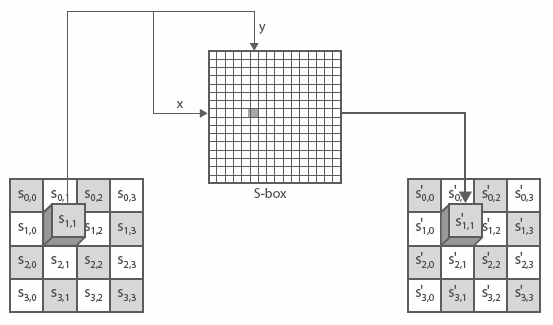
\includegraphics[scale=0.65]{assets/subbytes.png}
		\caption{SubBytes үйлдэл}
		\label{fig:subbytes}
	\end{figure}
	\item \textbf{ShiftRows:}
	\begin{itemize}
		\item 1-р мөрийг шилжүүлэхгүй
		\item 2–р мөрийн байтуудыг зүүн тийш 1 байт шилжүүлнэ
		\item 3–р мөрийн байтуудыг зүүн тийш 2 байт шилжүүлнэ
		\item 4–р мөрийн байтуудыг зүүн тийш 3 байт шилжүүлнэ
		\item Тайлах үйлдлийг хийхдээ баруун тийш шилжүүлэх үйлдлийг хийнэ
	\end{itemize}
	\begin{figure}[h]
		\centering
		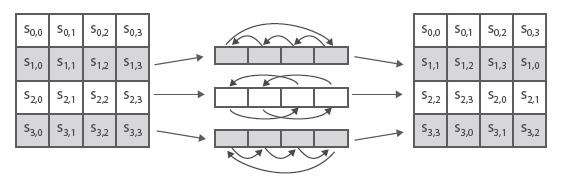
\includegraphics[scale=0.6]{assets/shiftrows.png}
		\caption{ShiftRows үйлдэл}
		\label{fig:shiftrows}
	\end{figure}
	\item \textbf{MixColumns:}
	\begin{itemize}
		\item Багана бүр тус тусдаа холигдоно
		\item Багана болгоны харгалзаа байтууд хоорондоо солигдоно
	\end{itemize}
	\begin{figure}[h]
		\centering
		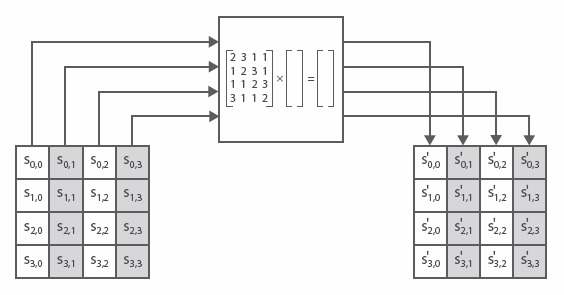
\includegraphics[scale=0.6]{assets/mixcolumns.png}
		\caption{MixColumns үйлдэл}
		\label{fig:mixcolumns}
	\end{figure}
	\item \textbf{AddRoundKey:}
	\begin{itemize}
		\item 128 бит XOR үйлдлийг циклийн түлхүүрт ашиглана
		\item Тайлах үйлдэл хийх бол эсрэгээр гүйцэтгэнэ
	\end{itemize}
	\begin{figure}[h]
		\centering
		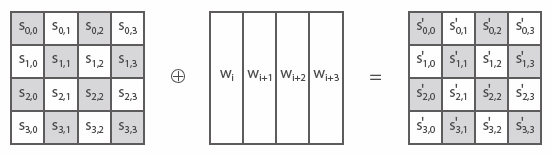
\includegraphics[scale=0.6]{assets/addroundkey.png}
		\caption{AddRoundKey үйлдэл}
		\label{fig:addroundkey}
	\end{figure}
\end{enumerate}

\subsubsection{AES-ын нууцлалт, нууцын тайлалт}
\begin{enumerate}
	\item шифрлэх блок ба түлхүүрийн урт, мөчлөгийн тоог сонгох. Шифрлэх блок ба түлхүүрийн урт нь 128, 192, 256 байт байж болох бөгөөд мөчлөгийн тоо нь харгалзан 10, 12, 14 байна.
	\item Шифрлэх текст, түлхүүрийн матриц \textit{T, W, K}-г үүсгэнэ.
	\item Эцсийн мөчлөгөөс бусад мөчлөгийн \textit{T, W, K} матрицуудад \textbf{AES}-н үндсэн үйлдлүүдийг дэс дараалан хийнэ. Харин эцсийн мөчлөгт Mix Columns үйлдлийг хйихгүй.
\end{enumerate}
% 4x4 for matrix below
\begin{center}
	$\begin{bmatrix}
		b_{0} & b_{4} & b_{8} & b_{12} \\
		b_{1} & b_{5} & b_{9} & b_{13} \\
		b_{2} & b_{6} & b_{10} & b_{14} \\
		b_{3} & b_{7} & b_{11} & b_{15} \\
		\end{bmatrix}$
\end{center}

\chapter{Системийн зохиомж}